\documentclass{beamer}
\usetheme{Hannover}

\usepackage[utf8]{inputenc}
\usepackage[T1]{fontenc}
\usepackage{graphicx}
\usepackage{amsmath}
\usepackage{amssymb}
\usepackage{capt-of}
\usepackage{hyperref}
\title{An Introduction To Neural Networks}
\author{Adithya Nair}
\institute{The Journal Society, Amrita Vishwa Vidyapeetham}
\date{\today}

\begin{document}
\begin{frame}
\titlepage
\end{frame}
\section{Introduction}
\begin{frame}
  \frametitle{An Introduction}
  \begin{itemize}
  \item The Journal Society is a group of people coming together to discuss mathematic and scientific ideas in a rigorous fashion.
    \item  We also have sessions happening in parallel on Real Analysis, following Terence Tao's textbooks on Analysis.
  \end{itemize}
\end{frame}

\begin{frame}
  \frametitle{What \textit{are} neural networks?}
  A neural network is a function. It takes an input, and maps it to some output.
  \[f : \mathbb{R}^m \rightarrow \mathbb{R}^n\]
\end{frame}
\section{An Example}
\begin{frame}
  \frametitle{An Example}

  Let's say we had $M$ greyscale images of the digits $0 \cdots 9$ on a square. How do you make a computer recognize each digit.

\begin{figure}[ht]
  \centering
  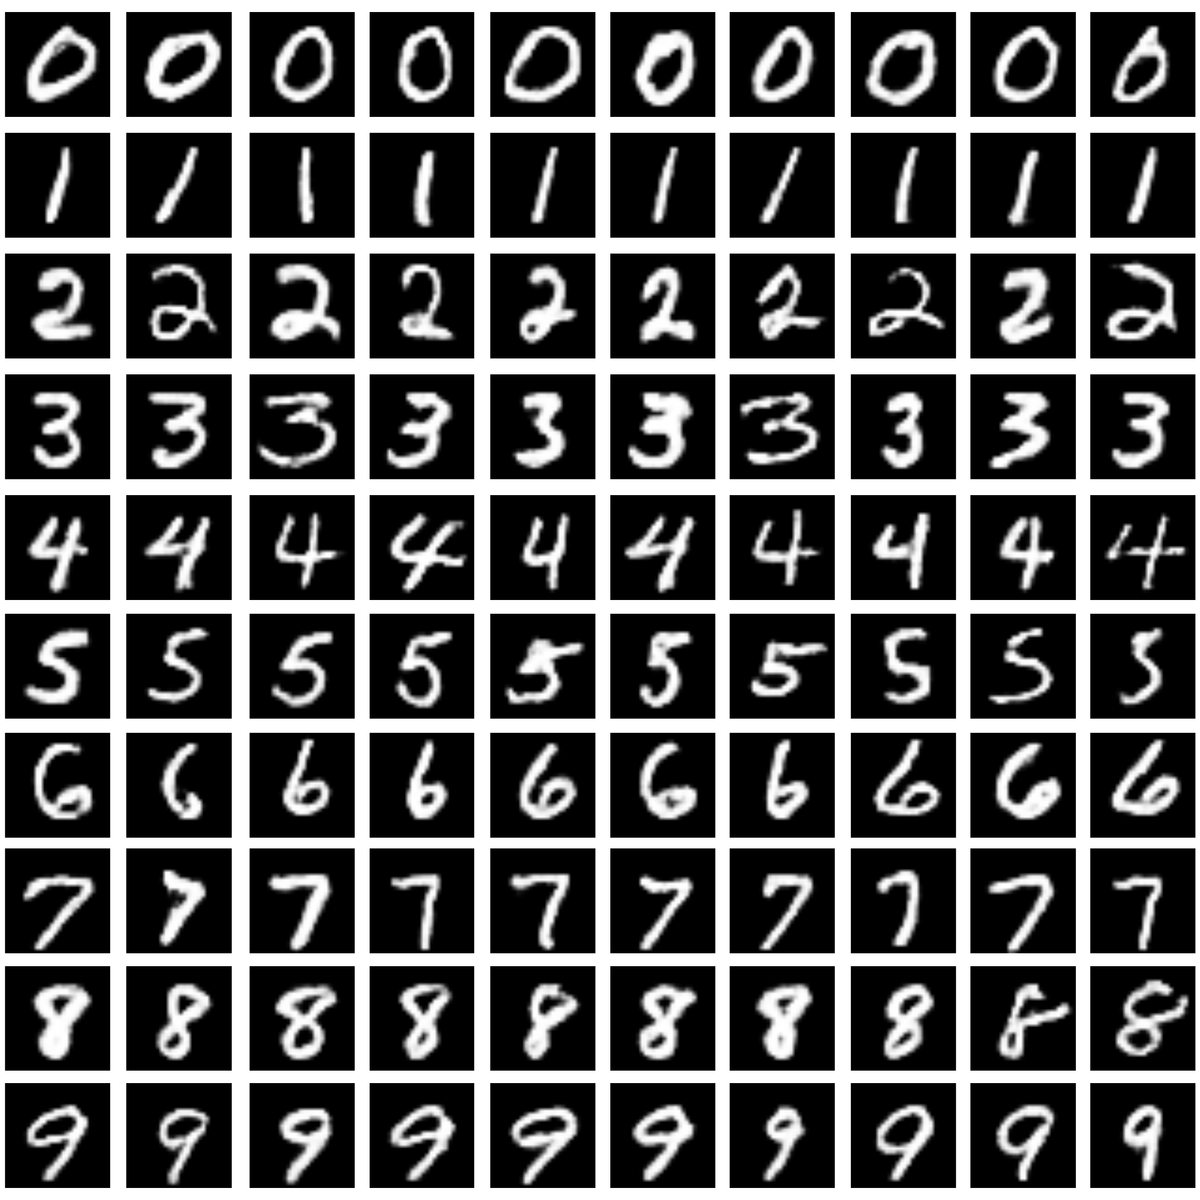
\includegraphics[width=0.5\textwidth]{figures/dataset-card.png}
  \caption{Each digit drawn out clearly}
\end{figure}

\end{frame}
\begin{frame}
  \frametitle{An  Example}
  \begin{enumerate}
\item Each image is a set of \(p\) pixels, or a vector \(\vec{v} = (v_1, v_2, \cdots , v_p)\). Each element \(v_i\) tells us how 'dark' or 'light' that pixel is. 0 is black, and 1 is white.
          \pause
          \item We have \(M\) vectors \(\vec{v}\) in \(p\) -dimensional space or \(\mathbb{R}^{p}\)
          \pause
          \item  We do have \emph{a} function \(f\) that can map these specific vectors \(v\) to an output in the discrete set \(\{0, \cdots , 9\}\).
  \end{enumerate}
\end{frame}

\begin{frame}
 \frametitle{The Problem}
 The function that maps these vectors cannot do this for \textbf{new} vectors.
 \pause
\linebreak
 We need a good ``rule''.
\end{frame}

\begin{frame}
\frametitle{Universality}
Neural networks are capable of \textbf{universal approximation}.
\end{frame}

\begin{frame}
\frametitle{The Big Picture}
Neural networks are compositions of simple functions.
$$F(v) = F_L(F_{L-1} \cdots F_2F_1(\vec{v})))$$

The reason they work so well, is that we are finding or computing the right parameters such that the output of this function matches the expected output as much as possible.

\pause

These parameters perform operations such as shifting, inverting and scaling functions that allows them to match real-world outputs in effective ways.

\pause
What are these `simple' functions?
\end{frame}
\begin{frame}
  \frametitle{Linear Functions}
 \[F(v): \mathbb{R}^p \rightarrow \mathbb{R}^{10}\]
 \begin{block}{Definition - Linear Functions Or Linear Maps}
A linear function, in linear algebra terms, means a mapping between two vector spaces $V \rightarrow W$ which preserves the operations of vector addition and scalar multiplication.

The function $f$ is such that,
\begin{enumerate}
\item  $f(u+v) = f(u) + f(v)$
\item $f(cu) = cf(u)$
\end{enumerate}
\end{block}

\end{frame}

\begin{frame}
  \frametitle{They Don't Work}
  Linear functions don't work well.
  \pause
 The input-output mapping of real world problems are rarely linear.
\end{frame}

\begin{frame}
\frametitle{Continuous Piecewise Linear Functions}
\begin{block}{Definition}
   A function $f(x)$ is said to be piecewise continuous on an interval $[a,b]$ if it is defined and continuous except possibly at a finite number of points $a\leq x_1 \leq x_2 \leq \dots \leq x_n \leq b$ Furthermore, at each point of discontinuity, we require that the left and right hand limits exists.
   \[
      f(x_k^-) = \lim_{x \rightarrow x_k^-} f(x); f(x_k^+) = \lim_{x\rightarrow x_k^+} f(x)
   \]
   At the ends of the domain, the left hand is ignored at $a$ and the right hand limit is ignored at $b$.
 \end{block}
\end{frame}
\begin{frame}
\frametitle{An Example Of Such Functions}
\begin{figure}[htbp]
\centerline{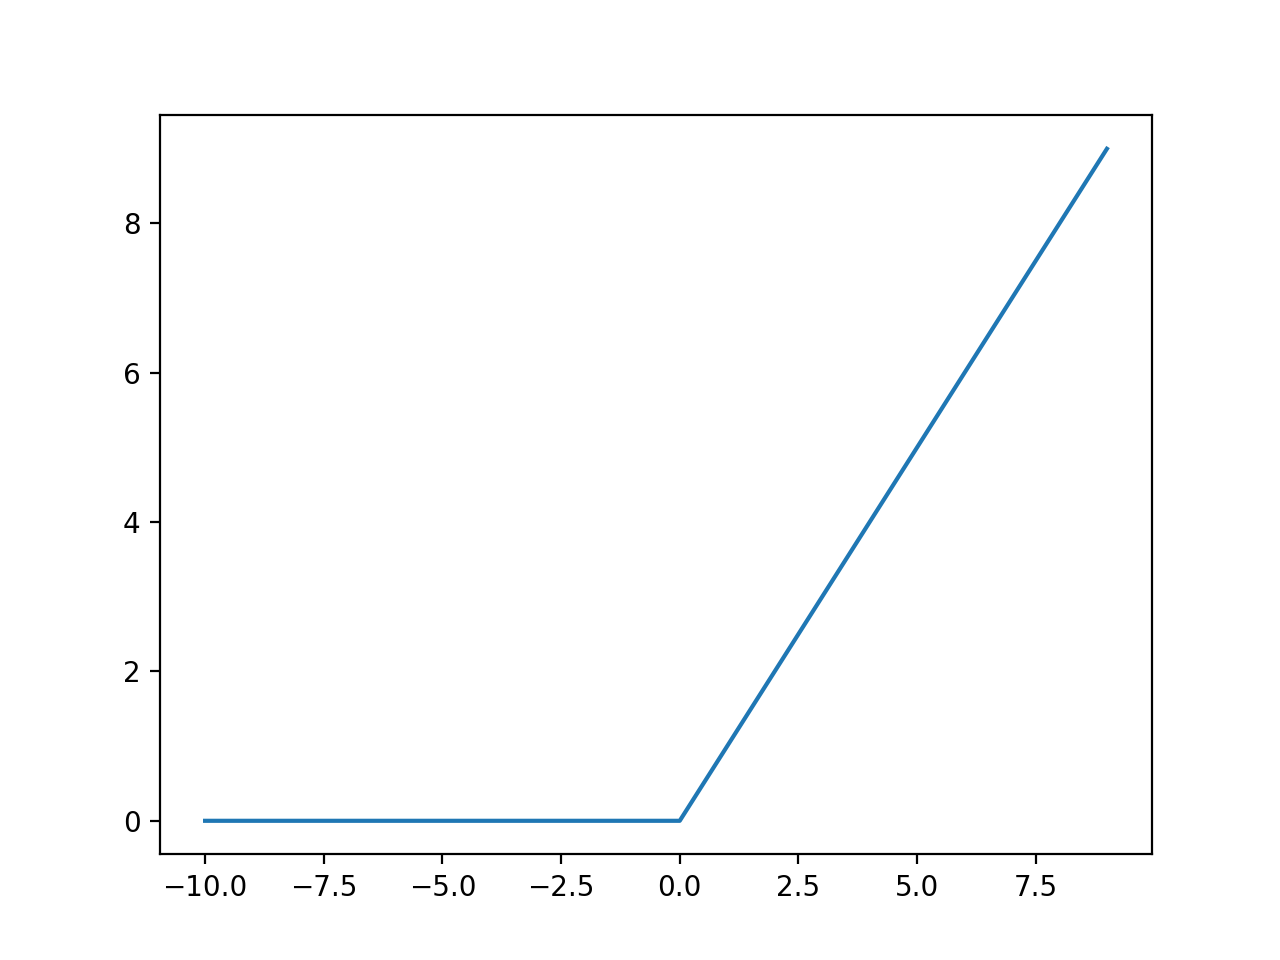
\includegraphics[width=0.65\textwidth]{figures/ReLU.png}}
\caption[The RELU function]{\label{fig:RelUActivation} The RELU (REctifier Linear Unit) function}

\[f(x) = \text{max}(x,0)\]
\end{figure}
\end{frame}
\begin{frame}
  \frametitle{Why Do They Work?}
\begin{quote}
``Linear for simplicity, continuous to model an unknown but reasonable rule and piecewise to achieve the nonlinearity that is an absolute requirement for real images and data.'' --- Gilbert Strang, Linear Algebra And Learning From Data (2019)
\end{quote}
\end{frame}

\begin{frame}
  \frametitle{Affine Functions}
  \begin{block}{Definition}
    An affine function is a function with a linear transformation as well as a translation.

    $$F(\vec{v}) = A \vec{v}+ b $$
\end{block}
\end{frame}

\section{A Small Introduction To Partial Derivatives}
\begin{frame}
  \frametitle{A Small Introduction To Partial Derivatives}
\begin{block}{Definition}
The derivative of a function dependent on multiple variables with respect to one of the variables, while the others are kept constant. For a function $f(x,y,\cdots)$,
$$\frac{\partial f}{\partial x} = f'_x$$
  \end{block}
  \end{frame}

\end{document}
